\documentclass[11pt,a4paper]{article}
\usepackage[margin=18mm]{geometry}\usepackage[T1]{fontenc}\usepackage{lmodern}\usepackage{microtype}\usepackage{xcolor}\usepackage{booktabs}\usepackage{tabularx}\usepackage{listings}\usepackage{tikz}\usetikzlibrary{arrows.meta,positioning}\usepackage[hidelinks]{hyperref}
\definecolor{codebg}{RGB}{246,247,249}\lstset{basicstyle=\ttfamily\small,backgroundcolor=\color{codebg},frame=single,breaklines=true,columns=fullflexible}
\title{Franka Panda Control Using MediaPipe Body Pose and Hand Gestures\\\large ROS 2 Humble, MoveIt Servo and Franka Hand}\author{Laboratory Project Guide}\date{16 September 2026}
\begin{document}\maketitle
\section{Purpose}This project extends the validated Franka Panda ROS~2/MoveIt setup with a camera-based human--robot interface. MediaPipe tracks the operator's body and hands. Right-arm body motion generates small Cartesian velocity commands for MoveIt Servo, while a thumb--index pinch controls the Franka gripper. All motion starts disabled.
\section{Architecture}
\begin{center}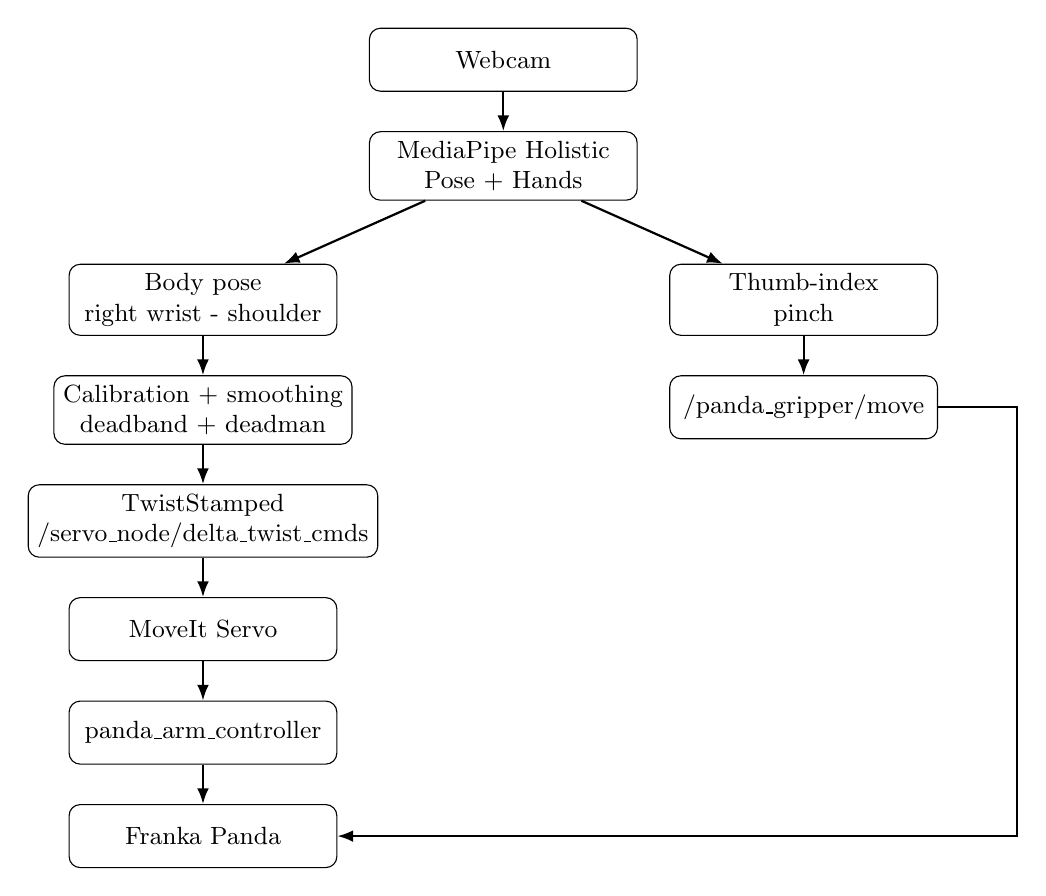
\begin{tikzpicture}[node distance=5mm and 8mm,every node/.style={font=\small},box/.style={draw,rounded corners,align=center,minimum width=34mm,minimum height=8mm},arr/.style={-{Latex[length=2mm]},thick}]
\node[box](cam){Webcam};\node[box,below=of cam](mp){MediaPipe Holistic\\Pose + Hands};\node[box,below left=8mm and 4mm of mp](pose){Body pose\\right wrist - shoulder};\node[box,below right=8mm and 4mm of mp](hand){Thumb-index\\pinch};\node[box,below=of pose](safe){Calibration + smoothing\\deadband + deadman};\node[box,below=of safe](twist){TwistStamped\\/servo\_node/delta\_twist\_cmds};\node[box,below=of twist](servo){MoveIt Servo};\node[box,below=of servo](ctrl){panda\_arm\_controller};\node[box,below=of ctrl](robot){Franka Panda};\node[box,below=of hand](grip){/panda\_gripper/move};
\draw[arr](cam)--(mp);\draw[arr](mp)--(pose);\draw[arr](mp)--(hand);\draw[arr](pose)--(safe);\draw[arr](safe)--(twist);\draw[arr](twist)--(servo);\draw[arr](servo)--(ctrl);\draw[arr](ctrl)--(robot);\draw[arr](hand)--(grip);\draw[arr](grip.east)--++(10mm,0)|-(robot.east);\end{tikzpicture}\end{center}
MoveIt Servo receives fresh timestamped Cartesian commands and is configured to output \texttt{JointTrajectory} messages to \texttt{/panda\_arm\_controller/joint\_trajectory}, with collision checking and singularity/joint-limit handling enabled.
\section{Gesture mapping and safety}
\begin{tabularx}{\textwidth}{@{}lX@{}}\toprule Input & Result\\\midrule Right hand toward/away camera & Panda X translation\\Right hand left/right & Panda Y translation\\Right hand up/down & Panda Z translation\\Left wrist above shoulder & Arm deadman enabled\\Left wrist lowered & Zero arm velocity\\Thumb-index pinch & Gripper closes to 0.04 m\\Thumb-index apart & Gripper opens to 0.08 m\\\bottomrule\end{tabularx}
The arm additionally requires \texttt{C} calibration and keyboard \texttt{A}. Default maximum Cartesian speed is 0.03~m/s. Angular commands are disabled. Gripper gestures are separately enabled with \texttt{G}.
\section{Installation}
\begin{lstlisting}
cd ~
unzip Franka_MediaPipe_BodyPose_HandGesture_Control.zip
cd Franka_MediaPipe_BodyPose_HandGesture_Control
conda deactivate
bash scripts/install.sh
\end{lstlisting}
The installer creates a MediaPipe virtual environment and builds \texttt{~/panda\_body\_servo\_ws}. It does not modify apt packages automatically.
\section{Terminal procedure}
In Franka Desk recover/unlock, activate FCI, clear the workspace and verify \texttt{ping -c 3 172.16.0.2}.
\subsection*{Terminal 1: Panda + MoveIt + gripper}\begin{lstlisting}
bash scripts/start_robot.sh
\end{lstlisting}
\subsection*{Terminal 2: MoveIt Servo}\begin{lstlisting}
bash scripts/start_servo.sh
\end{lstlisting}
\subsection*{Terminal 3: check and enable Servo}\begin{lstlisting}
bash scripts/check_system.sh
bash scripts/enable_servo.sh
\end{lstlisting}
Expected controller state is \texttt{joint\_state\_broadcaster active} and \texttt{panda\_arm\_controller active}. The earlier Panda test produced approximately 30~Hz joint states and successful gripper actions. The new Servo layer must be validated before normal use.
\subsection*{Terminal 4: MediaPipe}\begin{lstlisting}
bash scripts/run_dry_demo.sh
# after dry validation:
bash scripts/run_real_control.sh
\end{lstlisting}
\section{First real test}Press \texttt{C} while standing neutrally. Test the gripper first with \texttt{G}. Next press \texttt{A}; the arm still cannot move until the left wrist is above the left shoulder. Raise the left hand, move the right hand only a few centimetres, then lower the left hand to stop. If an axis is reversed, change its sign in \texttt{config/body\_control.json} only after returning to dry mode.
\section{Key configuration}\begin{lstlisting}
"max_linear_speed_mps": 0.03,
"body_deadband_m": 0.04,
"body_full_scale_m": 0.22,
"robot_x_from_body_z_sign": -1.0,
"robot_y_from_body_x_sign":  1.0,
"robot_z_from_body_y_sign": -1.0
\end{lstlisting}
\section{Stop}\begin{lstlisting}
# Q in camera window
bash scripts/stop_servo.sh
\end{lstlisting}
Then stop Servo and MoveIt with \texttt{Ctrl+C} and return the Panda to a safe state in Franka Desk.
\section{Validation status}ROS~2 hardware communication, MoveIt startup, the active Panda trajectory controller, joint-state streaming and gripper actions were already validated on the lab Panda. The body-pose-to-Servo layer is the next experimental integration and should be validated progressively: dry camera test, Servo checks, zero/small commands, then normal teleoperation.
\end{document}
